\documentclass{ximera}
\usepackage{sagetex}
%% handout
%% space
%% newpage
%% numbers
%% nooutcomes
 
%% You can put user macros here
%% However, you cannot make new environments

\graphicspath{{./}{module1Activity/}{module2Activity/}{module3Activity/}}

\usepackage{sagetex}
\usepackage{tikz}
\usepackage{hyperref}
\usepackage{tkz-euclide}
\usetkzobj{all}
\pgfplotsset{compat=1.7} % prevents compile error.

\tikzstyle geometryDiagrams=[ultra thick,color=blue!50!black]
 %% we can turn off input when making a master document
 
\outcome{}
\author{Darryl Chamberlain Jr.}
  
\title{Objective 2 - Identify Domain of Linear Model}
 
\begin{document}
\begin{abstract}

\end{abstract}

\maketitle
 
%%%%%%%%%%%%%%%%%%%%%
%%%  Objective 2  %%%
%%%%%%%%%%%%%%%%%%%%%

When modeling real-world phenomena, we are not normally looking at the entire domain of the linear function. First, let's think about different scenarios where we would have a restricted domain: 

\begin{itemize}
	\item Restricted Domain is a subset of the \textbf{Natural Numbers}
		\begin{itemize}
			\item Number of points scored in basketball/football/soccer.
			\item Number of tickets sold for an event.
			\item Number of tails when flipping a coin.
			\item Population of a city.
		\end{itemize}
	\item Restricted Domain is a subset of the \textbf{Integers}
		\begin{itemize}
			\item Number of points scored in golf. 
			\item Counting inventory (negative values for items sold).
		\end{itemize}
	\item Restricted Domain is a \textbf{\textit{Proper} Subset of the Real Numbers}
		\begin{itemize}
			\item Revenue (we normally only consider rounding to two decimal places).
			\item Time (if we only consider moving ahead in time).
			\item Grade Point Average.
		\end{itemize}
	\item \textbf{No Restricted Domain} 
		\begin{itemize}
			\item Time (if we can ``rewind" as negative time).
			\item Force of an object.
			\item Weight of an object.
		\end{itemize}
\end{itemize}

This list is not exhaustive, but meant as a way to get you to think why we might be considering a restricted domain. For the questions below, choose the restricted domain of the model. \textit{Note: We use ``Proper" to clarify that this is a smaller subset, since the Real numbers are technically a subset of the Real numbers.} 

%%% Domain is natural numbers
\begin{question}
Kappa Delta is hosting an all-you-can-eat pancake fundraiser to support the prevention of child abuse. Adult (18+) tickets are \$10 and teen (10-17) tickets are \$5. Children under 10 are let in without a ticket. What is the restricted domain the model is reasonable under?

\begin{multipleChoice}
\choice[correct]{Subset of the Natural numbers}
\choice{Subset of the Integers}
\choice{Subset of the Rational numbers}
\choice{All Real Numbers}
\end{multipleChoice}

\begin{feedback}[correct]
We cannot sell partial or negative amounts of tickets. We also couldn't have sold more of one type of ticket than the total number sold, so the domain is not all Natural numbers. \textit{(For example, if the total number of tickets sold were 343, they couldn't have sold more than 343 Adult tickets. So our restricted domain is the set of Natural numbers up to 343.)}
\end{feedback}
\end{question}

\begin{question}
A ball is dropped from the top of Century Tower. The ball steadily picks up speed before hitting the ground. You want to figure out what the ball's speed is at a certain time. What is the restricted domain the model is reasonable under?

\begin{multipleChoice}
\choice{Subset of the Natural numbers}
\choice{Subset of the Integers}
\choice[correct]{Subset of the Real numbers}
\choice{All Real Numbers}
\end{multipleChoice}

\begin{feedback}[correct]
We see time, so we are thinking it will either be a proper subset of the Real numbers or all Real numbers. Since we are considering dropping a ball, we have a ``starting" time and do not model time after the ball hits the ground. Therefore, we are looking at a proper subset of the Real numbers. 
\end{feedback}

\end{question}

\begin{question}
Chemists commonly create a solution by mixing two products of differing concentrations together. For example, a chemist could have large amounts of a 10\% acid solution and a 30\% acid solution, but need a 10 liter 15\% solution. What is the restricted domain the model is reasonable under?

\begin{multipleChoice}
\choice{Subset of the Natural numbers}
\choice{Subset of the Integers}
\choice[correct]{Subset of the Real numbers}
\choice{All Real Numbers}
\end{multipleChoice}

\begin{feedback}[correct]
We can consider partial amounts of volume, so the restricted domain is either a proper subset of the Real numbers or all Real numbers. If the goal is getting a 10 liter solution, then we shouldn't need to mix more than 10 liters total between the two solutions. Therefore, we are looking at a proper subset of the Real numbers. 
\end{feedback}

\end{question}

\begin{question}
What is the restricted domain the model below is reasonable under?
\begin{figure}
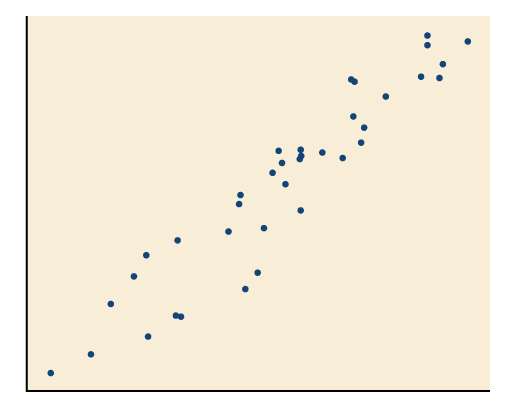
\includegraphics[scale=0.4]{positiveR.png}
\caption{\href{https://cnx.org/contents/mwjClAV_@8.12:6dX4RGdg@12/Fitting-Linear-Models-to-Data}{Scatterplot}}
\end{figure}

\begin{multipleChoice}
\choice{Subset of the Natural numbers}
\choice{Subset of the Integers}
\choice{Subset of the Real numbers}
\choice[correct]{All Real Numbers}
\end{multipleChoice}

\begin{feedback}[correct]
Our axes do not have any units, so we cannot be sure whether we would have a ``common sense" restriction (like time being positive). We can thus consider the domain as all Real numbers, \textbf{though the model may not be very predictive outside of the domain of values on the scatterplot}.
\end{feedback}

\end{question}

\begin{question}
What is the restricted domain the model below is reasonable under?
\begin{figure}
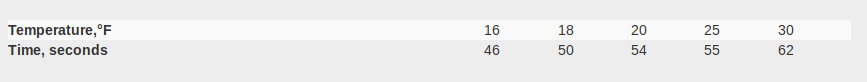
\includegraphics[scale=0.4]{temperature.png}
\caption{\href{https://cnx.org/contents/mwjClAV_@8.12:6dX4RGdg@12/Fitting-Linear-Models-to-Data}{Temperature over time (s).}}
\end{figure}

\begin{multipleChoice}
\choice{Subset of the Natural numbers}
\choice{Subset of the Integers}
\choice{Subset of the Real numbers}
\choice[correct]{All Real Numbers}
\end{multipleChoice}

\begin{feedback}[correct]
While the table only shows natural numbers, we know that temperature can be fractions and negative. We can thus consider the domain as all Real numbers, \textbf{though the model may not be very predictive outside of the domain of values on the table}.
\end{feedback}


\end{question}

\end{document}